\section{Qualidade de energia e eficiência}

\begin{frame}{Harmônicas: medida básica}
\small
\begin{columns}[T,onlytextwidth]
\column{0.50\textwidth}
\[
THD_I=100\frac{\sqrt{I_2^2+I_3^2+\cdots+I_n^2}}{I_1}.
\]
\begin{itemize}
\item THD não informa sozinho qual harmônica domina.
\item Analisar espectro e forma de onda.
\item Fonte, carga e impedância da rede determinam a distorção de tensão.
\end{itemize}
\column{0.48\textwidth}
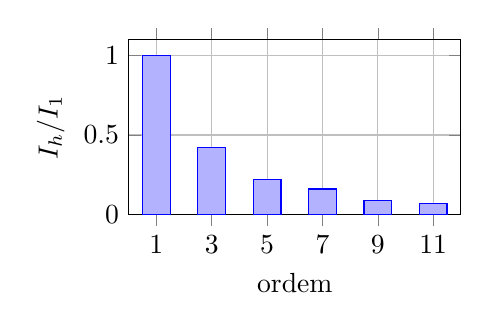
\begin{tikzpicture}
\begin{axis}[width=5.8cm,height=3.8cm,ybar,bar width=10pt,xlabel={ordem},ylabel={$I_h/I_1$},ymin=0,ymax=1.1,xtick={1,3,5,7,9,11},grid=major]
\addplot coordinates {(1,1)(3,0.42)(5,0.22)(7,0.16)(9,0.09)(11,0.07)};
\end{axis}
\end{tikzpicture}
\end{columns}
\end{frame}

\begin{frame}{Efeitos de harmônicas}
\small
\begin{columns}[T,onlytextwidth]
\column{0.49\textwidth}
\begin{itemize}
\item Aquecimento extra de cabos e transformadores.
\item Sobrecarga do neutro por harmônicas triplas.
\item Perdas adicionais em motores.
\item Erros/interferências em equipamentos sensíveis.
\end{itemize}
\column{0.49\textwidth}
\begin{itemize}
\item Ressonância com bancos de capacitores.
\item Correntes elevadas em capacitores.
\item Atuação indevida de proteção.
\item Redução de vida útil de componentes.
\end{itemize}
\end{columns}
\begin{caixaProjeto}[title=Mitigação]
Reatores, filtros passivos/ativos, transformadores adequados, arquitetura de alimentação, seleção de conversores e projeto do banco de capacitores -- sempre após medição/estudo.
\end{caixaProjeto}
\end{frame}

\begin{frame}{Correção de fator de potência}
\small
\begin{columns}[T,onlytextwidth]
\column{0.51\textwidth}
\begin{align*}
Q_c=P\left(\tg\varphi_1-\tg\varphi_2\right)
\end{align*}
\begin{itemize}
\item Reduz corrente reativa circulante a montante do ponto de compensação.
\item Pode liberar capacidade e reduzir perdas.
\item Não corrige distorção harmônica.
\end{itemize}
\column{0.47\textwidth}
\begin{caixaEx}
$P=\SI{100}{kW}$, $fp_1=0{,}78$, $fp_2=0{,}95$:
\[
Q_c\approx\SI{47}{kvar}.
\]
Em ambiente com VFD, verificar ressonância e considerar banco dessintonizado/filtro conforme estudo.
\end{caixaEx}
\end{columns}
\end{frame}

\begin{frame}{Gestão de demanda}
\small
\centering
\begin{tikzpicture}
\begin{axis}[width=10.6cm,height=4.5cm,xlabel={hora},ylabel={kW},xmin=0,xmax=24,ymin=0,ymax=110,grid=both,legend pos=north west]
\addplot[corPrim,thick,smooth] coordinates {(0,25)(4,20)(8,65)(10,80)(12,72)(14,88)(17,100)(18,96)(20,62)(24,32)};\addlegendentry{sem gestão}
\addplot[corAccent,thick,dashed,smooth] coordinates {(0,25)(4,20)(8,62)(10,72)(12,69)(14,75)(17,78)(18,76)(20,60)(24,32)};\addlegendentry{com gestão}
\end{axis}
\end{tikzpicture}
\begin{caixaObs}
Deslocar cargas flexíveis, limitar recarga de VE e coordenar climatização pode reduzir pico sem reduzir energia útil do processo.
\end{caixaObs}
\end{frame}

\begin{frame}{Medição: o que registrar}
\scriptsize
\begin{tabularx}{\textwidth}{>{\bfseries}p{4.0cm}X}
\toprule
Grandeza & Uso \\
\midrule
$V$, $I$, $P$, $Q$, $S$, fp & Estado operacional e balanceamento. \\
Demanda e energia & Custos, contratos e eficiência. \\
THD/espectro & Diagnóstico de cargas não lineares. \\
Afundamentos e elevações & Falhas de processo e qualidade de suprimento. \\
Interrupções & Continuidade e confiabilidade. \\
Temperatura e termografia & Conexões, sobrecarga e ventilação. \\
Eventos de proteção & Causa-raiz e seletividade. \\
\bottomrule
\end{tabularx}
\end{frame}

%=====================================================================
